\begin{frame}[fragile]{Tutorial: Custom two-site operators}

\begin{columns}

\begin{column}{5cm}

\begin{onlyenv}<1->

\begin{lstlisting}[language=JuliaLocal, style=julia, mathescape, basicstyle=\scriptsize\ttfamily]
import ITensors: op

function op(
  ::OpName"CRy",
  ::SiteType"S=1/2";
  $\theta$
)
  c = cos($\theta$/2)
  s = sin($\theta$/2)
  return [
    1 0 0  0
    0 1 0  0
    0 0 c -s
    0 0 s  c
  ]
end
\end{lstlisting}

\end{onlyenv}

\end{column}

\begin{column}{5cm}

\begin{onlyenv}<1-1>
~\\
~\\
Controlled-Ry (CRy) \\
rotation gate \\
~\\
CRy($\theta$) \\
~\\
~\\
~\\
~\\
~\\
~\\
~\\
~\\
~\\
~\\
\end{onlyenv}

\begin{onlyenv}<2->
\vspace*{0.0cm}
\begin{center}
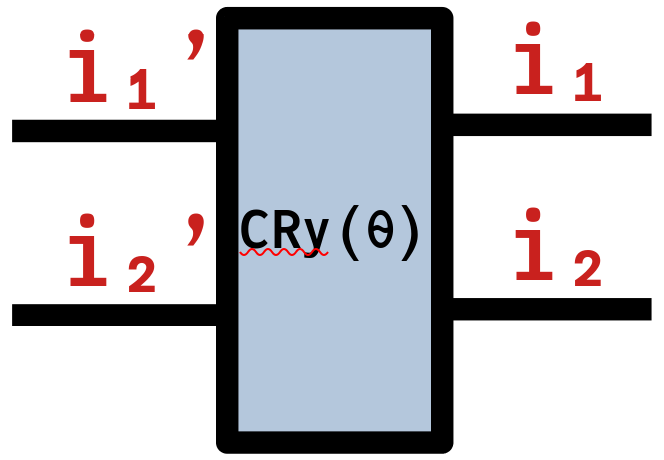
\includegraphics[width=1.0\textwidth]{
  slides/assets/CRy12.png
}
\end{center}
\vspace*{0.0cm}
\end{onlyenv}

\end{column}

\end{columns}

\end{frame}
